\chapter{Design}
In this chapter we will aim to explain the overall design of the experiment to be conducted and the underlying functionality of the various technologies involved in implementing Opportunistic Security in the MPLS network. We will also discuss on the Architectural design of the system and the reason for choosing the technologies.

%%%%%%%%%%%%%%%%%%%%%%%%%%%%%%%%%%%%%%%%%%%%%%%%%%%%%%%%%%%%%%%%%%% OS
\section{Opportunistic security (OS)}
Historically, the approach to internet security has always been with an 'all-or-nothing' attitude. Security protocols aims at either providing the service with full security or a complete hard failure. This discouraged many service providers from implementing the latest security tools to make their network secure. Service providers have a responsibility to maintain their Service Level Agreement (SLA) and as such will often end up disabling these security tools and pass clear text through their network whenever the connection becomes too slow or customers have trouble connecting to services.

Authentication, Confidentiality and Integrity are the three pillars of network security. Confidentiality and Integrity can be brought about using encryption techniques with hashing mechanisms. Authentication on the other hand has to be carried out on a peer to peer basis. The ability to authenticate any potential peer on the Internet requires an authentication mechanism that encompasses all such peers. No IETF standard for authentication scales as needed and has been deployed widely enough to meet this requirement \cite{rfc7435}.

Browsers, web services and network devices refer to the Public Key Infrastructure (PKI) model to authenticate their peers or web services. Implementation of the PKI has its own additional costs and burdens and considering the large number of Certificate Authorities (CA) that provide this service on the internet, many service providers have trust issues with regards to the CAs. This may lead to disagreement between peers in the network that are trying to connect to each other.

Thus if authentication of nodes in a network becomes optional, where the system can run normally with plain text if authentication cannot be easily attained then the network system is more likely to implement Encryption in majority of its links. This way the approach to network security changes from 'security being default and anything less than that as degraded security' to 'No protection being default and anything more than that is an improvement'

"Opportunistic Security" (OS) is defined as the use of cleartext as the baseline communication security policy, with encryption and authentication negotiated and applied to the communication when available \cite{rfc7435}. The aim of OS security is to implement encrypted and authenticated communication between peers whenever they are capable else only encrypted communication without authenticating the users or just clear text communication.

OS is not intended as a substitute for authenticated, encrypted communication when such communication is already mandated by policy (that is, by configuration or direct request of the application) or is otherwise required to access a particular resource. In essence, OS is employed when one might otherwise settle for cleartext .

\subsection{OS in MPLS}
As proposed in \cite{mpls-os-internet-draft} the basic requirement in MPLS OS is to provide a way to encrypt data passing between two MPLS switches by doing a key exchange between them to create a session key using which the encryption can be carried out. The key exchange between the LSRs is to be carried out using the Diffie-Hellman key exchange. Using the key values agreed after the Key exchange we encrypt the flowing packets using Advanced Encryption Standard (AES) cryptographic algorithm. To enable authentication of the peers as well in the encryption it is suggested to use AES in Galois/Counter Mode (GCM).

\subsubsection{Diffie-Hellman Key Exchange}
Diffie-Hellman Key Exchange is a way of sharing secret information between 2 nodes over an insecure channel. It was developed by Martin Hellman, Whitfield Diffie and Ralph Merkle. Using this protocol the 2 nodes agree on a secret symmetric key which can be later used in encrypting the sensitive data that is to be communicated.

The Diffie-Hellman key exchange is modelled based on the Internet Key Exchange Protocol Version 2 as specified in the RFC \cite{rfc7296}.

\subsubsection{Advanced Encryption Standard - Galois/Counter Mode (AES-GCM)}
AES is a symmetric blockcipher algorithm established by the U.S. National Institute of Standards and Technology in 2001. It was developed by Vincent Rijmen and Joan Daemen who won the NIST conducted AES selection process. AES is able to handle block encryption of sizes 128, 192 and 256 bits. It is expected to provide data security for 20-30 years and is free to use for all devices.

GCM is an Authenticated Encryption with Associated Data (AEAD) mode which is a form of encryption that simultaneously provides data confidentiality, integrity and authenticity. It extends AES's encryption functionality to incorporate Authentication and Data Integrity as well. GCM is widely adopted because of its efficiency and parallel processing. Unlike cipher block chaining whose pipeline operations bottle neck its efficiency, GCM makes efficient use of its instruction pipeline to provide high speed operations using parallel processing.

The Data packet in the MPLS OS must be encrypted with AEAD-AES-GCM-128 encryption algorithm based on the specifications mentioned in the \cite{rfc7296}.

\subsection{MPLS Packet Encryption}
The MPLS packet is encrypted using AES-GCM encryption algorithm whose Key and Initialization Vector are determined by the initial Diffie-Hellman Key exchange carried out between the two participating end-to-end LSRs in the MPLS network. The encryption state of the MPLS packet is identified by the addition of a special purpose MPLS label called the MPLS Encryption Label (MEL). The bottom of the stack of the MEL is set to 1 and should be followed by a 4 byte Pseudowire control Word (CW).

As specified in the \cite{rfc7296} the packet counter nonce used in the AES-GCM needs to be managed properly for successful Encryption and Decryption on the LSRs. The initial nonce value is derived from the HMAC-based Key Derivation Function (HKDF) output at key agreement time and the counter is incremented by one for each packet encrypted on the sending side and by one for each packet successfully decrypted on the receiver side \cite{mpls-os-internet-draft}.

The CW carries the low-order 16 bits of the nonce which helps the receiving LSR to identify any dropped packets or mismatch in the IV packet counter. The receiving LSR can then update the counter or resynchronize the counter to successfully decrypt the next incoming packets. The receiving LSR can raise alerts if more than 65536 packets are lost as the LSR will face a decryption failure, thus it is advisable to implement small window size to accept mismatched counters, beyond which the LSR will stop further decryption attempts to mitigate denial of service.

The AES-GCM generates a cipher packet which is slightly longer than the original packet. This is because of the additional authentication tag generated by the AES-GCM algorithm to provide authentication capabilities. The Receiving LSR will verify the authenticity of the encrypted packet as specified in \cite{rfc7296} by referring this authentication tag.

\begin{figure}[H]
       \centering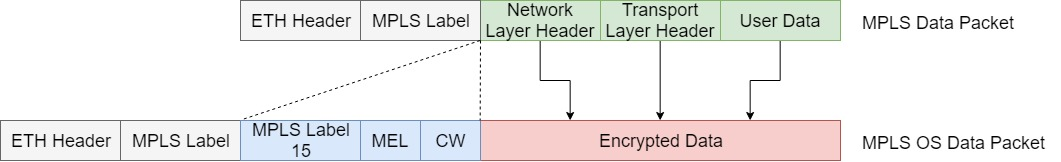
\includegraphics[width=\textwidth]{images/5_MPLS_Encrypted_Packet_Structure.jpg}
       \caption{MPLS OS Packet Structure}
       \label{fig:compbest}  
\end{figure}

Figure 2.1 shows the format of a normal MPLS packet with the MPLS with OS packet. In the normal MPLS packet an MPLS label with its bottom-of-stack (S) value 1 is pushed on top of the payload. Subsequent MPLS labels can be pushed over each other with values S = 0. Before transmission on the network the final Layer 2 header is pushed on top of the top MPLS label. In the MPLS OS data packet, the structure slightly changes. The Layer 2 header and the top MPLS label stays the same. The structure is then followed by the MPLS label with value 15. The value 15 informs the LSR that following this packet is a special purpose MPLS label. Then comes the MEL followed by the CW containing the low-order 16 bits of the nonce. The remainder of the packet is encrypted and contains the rest data of the packet.

\subsubsection{MPLS Encryption Label (MEL)}
The MPLS Encryption Label is a normal label stack entry carrying an extended special-purpose label with a value from the experimental range 240-255 \cite{mpls-os-internet-draft}. The structure of the MEL is same as that of the traditional MPLS Label. The values of the contents of the label is what differentiates the MEL from the traditional MPLS labels.

\subsubsection*{Label}
Considering this idea is still under experimentation no special purpose label value is yet assigned by the Internet Assigned Numbers Authority (IANA). The value however must be selected from the experimental range of 240-255

\subsubsection*{TC}
The TC field should be set to the value of the unencrypted label stack entry directly preceding the the MEL else it should be set to 0.

\subsubsection*{S}
The MEL should always be the bottom of the MPLS stack and thus its value S should always be 1.

\subsubsection*{TTL}
The TTL should ideally be set to 2 for end-to-end MPLS OS encryption to prevent the encrypted packets from being forwarded beyond the decrypting LSR.

\subsubsection{Control Word (CW)}
An LSR may tend to inspect the contents of an incoming packet to analyze its underlying protocol eg. check if it is IP and forward it via normal IP routing if so configured. The presence of the CW along with the MEL informs the receiving LSR that the contents of the MPLS packet is not of any standard protocol and thus cannot be inspected.

\begin{figure}[H]
       \centering
\includegraphics[width=\textwidth]{images/6_Code_Word.jpg}
       \caption{Pseudo-Wire Control Word Structure}
       \label{fig:compbest}
\end{figure}

Figure 2.2 shows the internal structure of the CW as specified in \cite{mpls-os-internet-draft}.
\subsubsection*{0000}
The Value of the first 4 bits of the CW is set to 0000 to identify it as an MPLS Payload \cite{rfc4385}.

\subsubsection*{Flags}
The Flags field is treated as a four-bit number. It contains the key-id that identifies the algorithm and key as established through configuration or dynamic key exchange \cite{mpls-os-internet-draft}.

\subsubsection*{Fragmentation FRG}
FRG indicates Fragmentation, MPLS OS doesn't support fragmentation of the Data packets and as such the FRG should always be set to 0.

\subsubsection*{Length}
Length is set to 0 and should be ignored by the receiving LSR

\subsubsection*{Sequence Number}
This field contains the low-order 16 bits of the nonce that is currently being used for the agreed encryption parameters. It is indicative of the counter used in the AEAD-AES-GCM encryption which the receiving LSR can use to check it its counter is correct and if it can go ahead with the decryption.

\section{Technologies Involved}
Considering the experimental nature of this project a proper base architecture needs to be designed to cover all the requirements of the experiment. This architecture will form the blueprint on which the technologies involved will be implemented to mimic the behavior of the MPLS network with and without the OS as close to the real life behavior as possible.

The ideal controlled test bed for this project should involve a virtualized environmental system on which network routers could be set up. The building up and tearing down of the network should be quick and clean so as to prevent long loading times or incomplete setting changes in the network settings even before the experimentation could begin. The virtualized routers involved should have all the basic MPLS functionality required for proper implementation of the MPLS network. The Routers should also be able to process the data packets at the kernel level so as to get readings as close to real-life routers as possible without any latency added due to the implemented technology or userspace processing. Secondly the Router functionality should be configurable to implement the OS functionality into the switches.

Based on these requirements the following technologies were chosen to implement the MPLS OS experiment.

\subsection{Mininet}
Mininet is a technology that can create realistic virtual network on a single machine. It is able to run real kernel and application code to provide authentic network behavior in a virtualized form. It has support for various switches all set up in a Software Defined Network Architecture. Mininet can yield a more efficient use of time and resources compared to other workflows. It provides a local environment for network innovation that complements shared global infrastructure \cite{lantz2010network},

Mininet is used for a wide variety of cases such as optimization of topology designs, tutorials for various network technologies, demonstrations, Regression Suits and most importantly Prototyping \cite{lantz2010network}. Mininet has the capacity of rapid and simplified prototyping, the applicability safety, the possibility of sharing results and tools at zero cost \cite{de2014using}.

\begin{figure}[H]
       \centering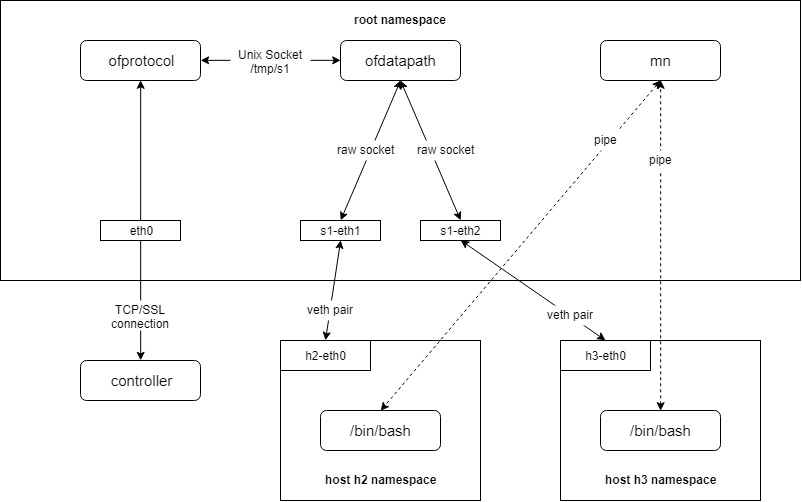
\includegraphics[width=\textwidth]{images/7_Mininet_Emulation.jpg}
       \caption{Mininet Emulation}
       \label{fig:compbest}
\end{figure}

Figure 2.3 \cite{lantz2010network} has described a basic architecture of how Mininet create a virtualized network with kernel functionality. Mininet creates a virtual network by placing host processes in network namespaces and connecting them with virtual Ethernet (veth) pairs.

\subsection{OpenVSwitch (OVS)}
OVS is a multi-layer Virtual Switch technology used to implement the functionalities of a hardware switch in a virtualized manner. It is designed for network automation  on a large scale using programmatic extension, while still supporting standard management interfaces and protocols (e.g. NetFlow, sFlow, IPFIX, RSPAN, CLI, LACP, 802.1ag) \cite{OVS}.

OpenVSwitch works with most hypervisors and container systems, including Xen, KVM, and Docker. OpenVSwitch also works “out of the box” on the FreeBSD and NetBSD operating systems and ports to the VMware ESXi and Microsoft Hyper-V hypervisors are underway \cite{pfaff2015design}. It is designed to be flexible and portable and lies inside the hypervisor to provide connectivity between the virtual switch and the physical interface. Figure 2.4 describes the architecture of OVS.

\begin{figure}[H]
       \centering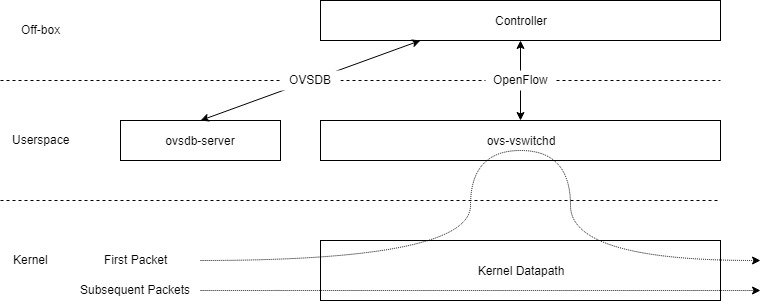
\includegraphics[width=\textwidth]{images/8_OVS_Architecture.jpg}
       \caption{OVS Architecture}
       \label{fig:compbest}
\end{figure}

OpenVSwitch relies on 2 major components for forwarding packets in a network. The ovs-vswitchd which is a daemon that lies in the userspace of the system and the smaller datapath kernel module. The ovs-vswitchd daemon is different in different operating system environment however provides the same functionality, the data path kernel module on the other hand is written especially to function at the kernel level.

Figure 2.4 explains how the components of the OpenVSwitch interact with each other. A packet which arrives on the interface of a physical or virtual NIC is passed onto the datapath kernel module. The datapath kernel module will do either of the following things: Forward the packet based on the flow logic instructed by the ovs-vswitchd or pass it to the ovs-vswitchd to await instructions on what actions to take on such types of packets.

\subsubsection{Kernel Forwarding}
The ovs-vswitchd daemon instructs the kernel datapath module how to handles packets of specific types or 'flows'. These instructions are called 'actions'. The actions may specify a range of functionalities like modification of packets, sampling, packet dropping, re-routing etc. The kernel datapath simply follows the flow rules set by the ovs-vswitchd and executes the actions mapped to them. The kernel datapath can store these flow rules from the ovs-vswitchd daemon in its cache to act similarly on similar types of data packets. If an incoming packet does not match any of the flows stored in the kernel modules cache, i.e a cache miss, then the module forwards it to the userspace instead.

\subsubsection{Userspace Forwarding}
When the kernel module forwards a packet to the userspace due to a cache miss the ovs-vswitchd daemon determines what actions are to be taken on the data packet. The Daemon then forwards the action to the kernel Datapath to cache it and handle future similar packets.

OpenVSwitch is commonly used as an SDN switch and the main way to control forwarding is OpenFlow. It leverages the use of Open Flow protocol to add, update, and delete flows in a switch's flow table. The ovs-vswitchd daemon receives these flow rules from an SDN controller. It also has a great support for MPLS from version 2.4 onwards where you have kernel support for MPLS packets upto a maximum of 3 label stack.

\subsection{OpenFlow}
Networks have become a critical part of our day to day lives from business to research. Due to the large number of equipment and protocol installation overhead along with the reluctance of network owners to experiment with their production network so as to not affect ongoing services, Network researchers have a difficult time in experimenting with new protocols and network technologies. This is where OpenFlow comes in. OpenFlow provides an open protocol to program the flowtable in different switches and routers \cite{mckeown2008openflow}. A network researcher is able to use OpenFlow protocol to control the flows in a flow table of all the switches inside the experimental network remotely and programmatically. This allows for easy and quick implementation of experimental setups which are ideal for research purposes.

An OpenFlow enables a switch to perform actions based on the experimental protocol. Using OpenFlow, a researcher experiments with his protocol by running it on a controller. The protocol will pick a route in the network of OpenFlow enabled switches and add the flow entry into all the switches in its path. The protocol can instruct the switches to encapsulate, drop, forward or push labels on top of packets like we do for MPLS LSRs. We can also set the flow rules to pick the type of data flows that pass through the Open flow enabled switch on which the actions are to be performed.

\section{Architecture of Experiment}
As Described in the previous chapter we will be implementing the MPLS OS system in a virtualized environment using Mininet, OpenVSwitch and OpenFlow technology. In order to simulate the MPLS OS structure and its effects on LSRs we need to design a network topology where we can analyze its overall effects in all use cases. Figure 2.5 Describes the topology of the network system we will be using to demonstrate the MPLS OS system.

\begin{figure}[H]
       \centering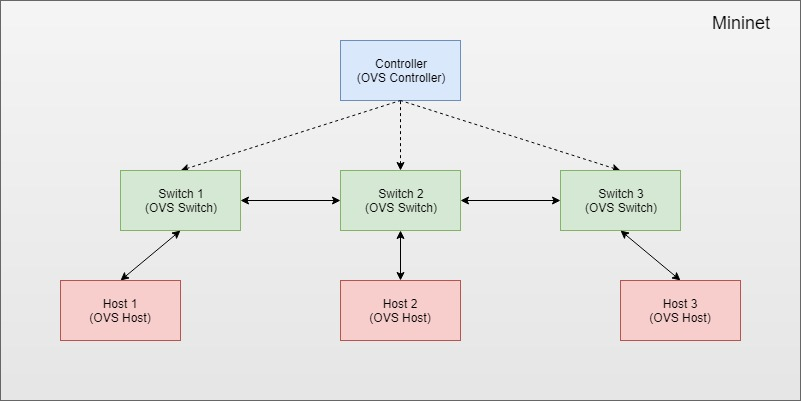
\includegraphics[width=\textwidth]{images/9_Topology.jpg}
       \caption{Network Topology for the Experiment}
       \label{fig:compbest}
\end{figure}

We will be using Mininet as our virtual network environment. The fast and clean network topology build up and tear down speed makes Mininet a good choice for setting up the virtual network environment. The Mininet version used in this experiment is version 2.2.1.

We will be deploying OpenVSwitch switches in the Mininet virtual network. Mininet has inbuilt support for setting up OpenVSwitches in its Virtual environment. The collaboration of both Mininet and OpenVSwitch makes both their use together in a system ideal for experimentation. The OpenVSwitch version used in this experiment is version 2.9.2

Flow rules and actions will be passed onto the OpenVSwitches using OpenFlow protocol. For this we need to setup an OVS controller which communicates the OpenFlow messages to all the OVS switches in the network. The OpenVSwitch Controller comes in built with Mininet and needs to be passed in the parameters for Mininet to setup in the network.

As shown in Figure 2.5 we will be setting up 3 switches (S1, S2, S3) in a linear topology. Each switch has its own host (H1, H2, H3) connected to it. Switch S1 has two interfaces s1-eth1 connected to host H1 and s1-eth2 connected to Switch S2 on its interface s2-eth2. Switch S2 has 3 interfaces s2-eth1 connected to host S2, s2-eth2 connected to Switch S1 on its s1-eth1 interface and s2-eth3 interface connected to Switch S3's s3-eth2 interface. Switch s3 has 2 interfaces, s3-eth1 connected to Host H3 and s3-eth2 connected to switch S2 on its s2-eth3 interface. Controller C0 will communicate the MPLS flow rules to all the three switches.

The Expected behavior of the system in normal MPLS process will be as follows:
\begin{enumerate}
\item Host 1 will ping an ICMP packet to Host 3
\item The packet will be first forwarded to Switch S1 at its s1-eth1 interface
\item S1, based on the flow rules that we will pass via the controller, will push an MPLS label on top of the packet and forward the packet along s1-eth2 interface.
\item Based on the linkage, S2 will receive the data packet. S2 will read the MPLS header value and forward it along its s2-eth3 interface.
\item Based on the linkage, S3 will receive the data packet. S3 will then pop the MPLS header and forward the normal ICMP packet to H3 via its s3-eth1 interface.
\item H3 will reply to the ICMP packet following the reverse path. the only difference being that now S3 will push the MPLS label and S1 will pop it at the end
\end{enumerate}

The Expected behavior of the system in MPLS OS process will be as follows:
\begin{enumerate}
\item Host 1 will ping an ICMP packet to Host 3
\item The packet will be first forwarded to Switch S1 at its s1-eth1 interface
\item S1, based on the flow rules that we passed via the controller, will first Encrypt the payload using AES-GCM encryption algorithm the keys and IV of which, for the scope of this project, are currently hard coded. After encryption the CW with the low-order 16 bits of the nonce is pushed on top of the Data packet. Then the MEL is pushed on top. A normal MPLS with value 15 is then pushed on top of the MEL completing the MPLS OS data packet which is then forwarded onto the s1-eth2 interface
\item Based on the linkage, S2 will receive the OS data packet. On parsing the Data packet S2 should stop any further inspection or hash checking functions on the underlying encrypted data. S2 should just read the MPLS header value and forward it along its s2-eth3 interface.
\item Based on the linkage, S3 will receive the data packet. S3 will then pop the MPLS header with the value 15. It will then read the MEL value and pop it, expecting the next header to be the CW. S3 will the compare its low-order 16 bits of the nonce value with the one present in the CW. If it is a match then the counters are correct and s3 can proceed with the decryption. If not then S3 will update its counter to continue decrypting the next oncoming packets. Once successfully decrypted S3 will then forward the normal ICMP packet to H3 via its s3-eth1 interface.
\item H3 will reply to the ICMP packet following the reverse path with encryption on S3 and Decryption on S1.
\end{enumerate}

The Diffie-Hellman Key exchange required to initialize the Symmetric Encryption Key and the Initialization vector for the AES-GCM encryption Algorithm is not implemented in this experiment and as such these values are currently hard coded into the system and can be later replaced with further development on that part. This experiment currently only demonstrates the encryption functionality of the OS and how the implementation of the OS Encryption affects the performance of the overall system.

